\lab{Algorithm}{Pseudorandom Number Generators}{Pseudorandom Number Generators}
\label{lab:PRNG}

\objective{Learn about the strengths and weaknesses of a few a pseudorandom number generators}

\section*{Random Numbers}
Lotteries, most board games, and statistics need random numbers.
In real life, we roll dice, take balls out of a bag, or spin a wheel.
Computers are, by nature, deterministic, meaning that they do exactly what they are told.
Because of this, random number generation on a computer can be difficult.
We can have a device measure a random process and use the data to generate random numbers, 
But such sampling is often too slow and too expensive for practical use.
Pseudorandom number generators (PRNGs) are a common solution to this problem.
The numbers are not truly random, but they are based on a complex formula that makes them look ``random."
For convenient use, these generateors must also run quickly.
The goal is to have something that is fast and looks random.

There are many different algorithms for developing pseudorandom numbers.
Robert R. Coveyou titled an article ``The generation of random numbers is too important to be left to chance."
There has been much study about different PRNGs.
This lab will cover two of them: Linear Congruiental Generators and The Mersenne Twister.

\section*{Linear Congruential Genterators}
Linear Congruential Generators (LCG) are one of the oldest ways of generating random numbers.
The Generator is defined by the recurrence relation:
$X_{n+1}=(a*X_n + c)$ mod $m$ where

\begin{itemize}
\item $X$ is a sequence of pseudorandom values, and
\item $m$, $0<m$ is the modulus
\item $a$, $0<a<m$ is the multiplier
\item $c$, $0\leq c<m$ is the increment
\item $X_0$, $0\leq X_0 <m$ is the seed
\end{itemize}

each of these are integer constants.

\begin{problem}
Write a LCG that produces an array of pseudorandom numbers between $0.0$ and $1.0$.
Let the arguments be size of the array and let a, c, mod, and seed be optional arguments.
I recommend $a=1103515245$, $c=12345$, $m=2^{31}-1$, and $seed=4329$ as the default values.
\end{problem}

\begin{problem}
Write a LCG that produces an array of pseudorandom numbers of integers between two input arguments.
Do it by calling your algorithm from problem one and multiplying it by the values and casting the array as an int using the .astype() function.
Let the arguments be size of array and the two integers.
Let a, c, mod, and seed continue to be optional arguments.
\end{problem}

One easy way to ``see" if your generator is random is to look at a bitmap of the output.
In python, use the plt.imshow() function to see a bitmap of the array produced by your LCG.
Resize your output to be $512 \times 512$.

\begin{figure}

\includegraphics[width=.4\textwidth]{PRNG1.png}
\caption{
The bitmap with $a=3$, $c=2$, $m=2^{16}$.
There is a clear pattern in the random numbers.}
\end{figure}

\begin{problem}
For what values of $a$, $c$, and $m$ does your LCG have a visible pattern.
\end{problem}

This method is not rigorous, but there are several other ways to test the randomness of your output.

The length over which your random number generator repeats is called the period.
The period is at most m, but it may be shorter based on the values of a and c.
 
\begin{comment}
According to the Hull-Dobell Theorem (TO DO: find a source), a LCG will have a full period if and only if, 
1. $c$ and $m$ are relatively prime,
2. $a-1$ is divisible by all prime factors of $m$,
3. $a-1$ is a multiple of 4 if $m$ is a multiple of 4

\begin{problem}
Test values of $a$,$c$, and $m$ that fit these requirements. 
\end{problem}
\end{comment}

This algorithm is used as the default random number generator in Java, and C++ and is still used in a wide variety of situations.

\section*{Mersenne Twister}
\begin{comment}
(TO DO: decide how much of  this we want to keep) All numbers can be represented in bits as a base two number.
Computers are optimized to work with numbers in that manner.
The operators XOR, OR, and AND work on the bit representation of two numbers.

AND - if both numbers have a 1 in the ith place then the ith place is 1.
Otherwise the ith place is 0.

OR - if one or both numbers have a 1 in the ith place then the ith place is 1.
Otherwise the ith place is 0.

XOR - if only one of the two numbers has a 1 in the ith place then the ith place is 1.
If both or neither of the numbers has a 1 in the ith place, the ith place is 0.

In addition you can shift the bitwise number over a number of values.
For example, shifting 10100 to the right by one yields 1010 and shifting it to the left by one yields 101000.
This is really just division and multiplication by 2.
This can be done by $\ll$ and $\gg$ in python. 
\end{comment}

The Mersenne twister PRNG does a series of bitwise operations to generate random numbers.
The Random class in python uses the Mersenne twister algorithm. 

\begin{problem}
Look at the bitmap of output of \li{np.random.rand(512,512)}.
Can you see any patterns?
\end{problem}

\section*{Randomness Tests}
There have been statistical tests devised for measuring the quality of a random number generator. One is these is the overlapping permutations test. Analyze sequences of five consecutive random numbers. The 120 possible orderings should occur with statistically equal probability.

\begin{problem}
Use the overlappng permutations test to see how random python's random number generator is compared to the LCG you wrote in problem 1.
Create a bar graph with 120 bins, one for each ordering, to view graphically the difference.
\end{problem}

\section*{Blackjack}
\begin{figure}
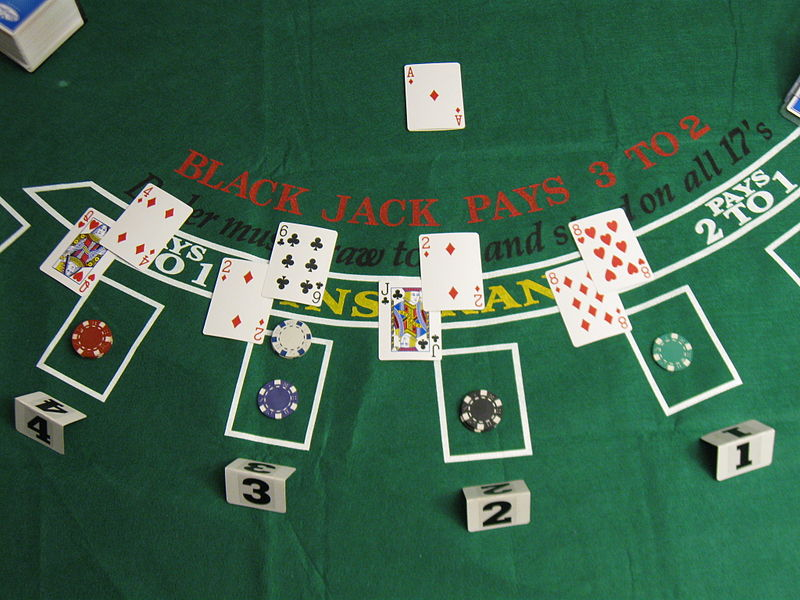
\includegraphics[width=\textwidth]{Blackjack_game_1.jpg}
\caption{Initial Round of a BlackJack game.}
\end{figure}

Black Jack is a card game that involves the use of randomness.
The game is simple.
The dealer deals the player and himself each two cards.
He flips over his first card so that the player can see it.
The player has to choose to take another card ("hit") or not ("stand").
If the player hits he gets another card and again has the choice to hit or stand.

The goal is to get your hand to be at or as close to 21 without going over.
Face cards are worth 10 points.
Aces can count either as 11 or 1.
The value of all other cards are equal to number on the card.

Once the player has decided to stand the dealer flips over his second card and deals himself cards until his hand value is 17 or greater. 

If the player value goes above 21 he automatically loses.
If his value is 21 and below and dealer has above 21 then the player wins.
If they both have 21 or under than the player with the hand of highest value wins.
If both hands have the same value, the game is a tie.

\section*{Shuffling Algorithms}
One use of Pseudorandom Number Generators (PRNGs) is to shuffle cards.
The main goal of these algorithms is that the card order be random--so that no single player has an advantage based on order.
Often, as strange as it may seem, online gambling sites will post their shuffling algorithms online.
The only things they do not post are their seed values.
Often the time in milliseconds from midnight is used as the seed value.

John von Neumann said ``Anyone who considers arithmetical methods of producing random digits is, of course, in a state of sin."
As seen in the last lab, weak PRNGs are periodic and are predictable once a few outputs are known.
This lab will have you break blackjack based on a weak PRNG.

\section*{Cracking Blackjack}
For these next problems you will need four files that are provided with this lab: BlackHard.py, BlackEasy.py, bjHelp.py, and bjDump.py.
BlackHard.py and BlackEasy.py are programs that run games of Blackjack that use a Linear Congruentail Generator (LCG) to shuffle the cards.
They generate 52 random numbers and then use the argsort of those numbers as the ordering of the cards.
The parameters for BlackEasy.py are a$=2521$, c$=13$, mod$=2^{16}$.
For BlackHard.py they are a$=25214903917$, c$=11$, mod$=2^{48}$.

In order to play them type \li{python <<filename>> <<numberofgames>>} in your command line.
Both use seeds based on the time, using \li{ (int)(time.time())}, which is the number of seconds from the start of the epoch cast as an integer. However, BlackEasy.py further scrambles it's seed, which for our purposes is in an unknown fashion.
Cards are popped off the deck one at a time, first one to the player, one to the dealer, one to the player, and one last one to the dealer. 

Initially 3 cards are visible (the last of the dealer's is face down) so our algorithms will deal with these first three cards, and the ordering (player,dealer,player) will be very important. 
After the first four cards are down the next cards are popped off in the order that they appear. 
After each game the deck is reshuffled.

bjHelp.py contains several functions to help you with the game's mechanics.
 Cards have a string representation ( '6diamond' for 6 of diamonds, 'Kclub' for king of clubs) and a number representation that determines their natural ordering. 
bjHelp.py has functions for generating the list  of cards and converting arrays to and from the string and integer representation of cards. 
Particularly useful is the function \li{Shuffle}, which returns the first n decks (or games) in integer representation in n arrays of 52 given the number of games, the LCG parameters, and a seed value.

bjDump.py has the functions \li{dumpEasy} and \li{dumpHard} to emulate the shuffling of the blackjack programs. 
Both take in the number of games as parameters. 
\li{dumpEasy} returns a list of shufflings based on a time based seed. 
\li{blackHard} also returns a list shufflings, as well as an appoximate time that the seed was chosen ( we'll explain the purpose of this later).

Your goal will be to do a sweep of seed values and cross check the decks produced by Shuffle against the first three cards from several games. 
The cross checking can be done using \li{numpy.where}. 
For example, the following can be used to find all the decks in \li{decks} whose first three cards are '6club','4club','3club'.

\begin{lstlisting}
np.where((decks[:,0:3]==bjHelp.convertToNum(['6club','Aheart','8spade'])).all(axis=1))[0]
\end{lstlisting}

The ouput is an array with all the indicies of the decks whose first three cards satisfy the conditions. 
The \li{all(axis=1)} is necessary to give a 1d array of truth values to \li{np.where}.
You will need to extend this command to match sets of three from more than one game, which amounts to merely an indexing issue.

\begin{warn}
Both BlackEasy.py and Black.py use functions that are incompatible with ipython. They need to run \li{python Black.py} in command line.
\end{warn}


\begin{problem}
Create a function to crack the shuffling algorithm of \li{blackEasy.py}. 
Have it take in a list of 3-tuples of the first three cards (in string representaion) of games and the number of games to play and then return the list of decks (in string representation) for the number of games specified. 
For example, you might give your function 4 lists of 3 cards each and have it calculate for 10 games. 
The output should then be an array of 10 by 52 strings. 
Although there may be more than one possible list of shuffling that satisfy the card orderings, in practice we will use enough hands to determine a unique list of shuffles. Just return by default the first list of shuffles in your result.

Although there are $52!$ different shufflings there are not that many possible seed values. 
From the parameters to the LCG, determine how many seed values there are and what values you should test.
There should be few enough that you can test all of them in a reasonable amount of time.

You can load up each result from bjHelp.Shuffle using the number of games specified for each seed value into an array and then use a call to \li{numpy.where} to find matches.
You will need to add in some more indices and perhaps another call to \li{all}.

You can use \li{bjDump.dumpEasy} to check that your function works. You should be able to determine the ordering in less than 5 games, usually in only one or two.
\end{problem}

\begin{problem}
Create a function to crack the shuffling algorithm of \li{blackHard.py}
This time there may be too many seed values for your computer to test in a reasonable amount of time. 
However, we know that the seed value is foolishly chosen by \li{(int)(time.time())}.
If we know at aproximately what time the seed is chosen, perhaps by syncing our time with whatever server we are working with, we can greately narrow down the possible space of seed values.
Have your function take in a list of 3-tuples of cards and the number of games, as before.
Have your function also take in an additional parameter for the approximate time that the seed was chosen.
If the time is not supplied, get it from \li{(int)(time.time())}.
Assume that whatever time you start with is within five minutes of the time the seed was chosen.

With this time, create a sweep as before of possible seed values and use \li{where} to find matches.
It may take more games than before to find a unique match.
You can check that your function works using \li{bjDump.dumpHard}.
\end{problem}
